% !TEX TS-program = xelatex
% !TEX encoding = UTF-8 Unicode
% !Mode:: "TeX:UTF-8"

\documentclass{resume}
\usepackage{zh_CN-Adobefonts_external} % Simplified Chinese Support using external fonts (./fonts/zh_CN-Adobe/)
%\usepackage{zh_CN-Adobefonts_internal} % Simplified Chinese Support using system fonts
\usepackage{linespacing_fix} % disable extra space before next section
\usepackage{cite}
% \usepackage{geometry}     % 可调整页边距
\usepackage[svgnames]{xcolor}    % 颜色支持
\usepackage{tcolorbox}    % 绘制彩色方框
\usepackage{graphicx}     % 插图
\usepackage{fontawesome5} % 图标包 (需在本地或 Overleaf 安装)
\usepackage[colorlinks=true,linkcolor=black,citecolor=blue,urlcolor=black]{hyperref}
\usepackage{xcolor}
% 仍保持超链接的常规设置 (colorlinks=true),文字本身可以是有色或无色
% \usepackage[colorlinks=true,linkcolor=blue,urlcolor=blue]{hyperref}
\hypersetup{
    colorlinks = true,
    urlcolor   = black,    % [paper]/[code] 链接的颜色
    linkcolor  = blue,
    citecolor  = blue
}

\usepackage{enumitem}        % 控制 enumerate/itemize 的间距

% 定义一些命令来简化对 [paper] [code] 超链接的调用
\newcommand{\PaperBoxLink}[1]{%
  \fcolorbox{cyan}{white}{%
    \href{#1}{\textcolor{blue}{[paper]}}%
  }%
}
\newcommand{\CodeBoxLink}[1]{%
  \fcolorbox{cyan}{white}{%
    \href{#1}{\textcolor{blue}{[code]}}%
  }%
}

% 定义一些奖项链接
\newcommand{\AwardBoxLink}[2]{%
  \fcolorbox{cyan}{white}{%
    \href{#1}{\textbf{#2}}%
  }%
}


% 如果想高亮自己名字,可加
\newcommand{\myname}[1]{\textbf{#1}} 
% 在条目中 \myname{蒋骞} 或 \myname{Qian Jiang} 这样写即可

\newcommand{\BoxedLink}[2]{%
  % #1: 显示的文字, #2: 链接 URL
  \fcolorbox{cyan}{white}{\href{#2}{#1}}%
}

\usepackage{tikz}
\newcommand{\FancyBadge}[2]{%
  \tikz[baseline=(txt.base)]{
    \node[
      rounded corners=3pt,
      fill=#1,
      text=white,
      inner sep=2pt,
      font=\bfseries
    ] (txt) {#2};
  }%
}
\newcommand{\MUSTqs}{\textit{工学博士}~\FancyBadge{teal}{QS 464}}

\begin{document}
\pagenumbering{gobble} % suppress displaying page number

  % 用一个两列结构:左侧文本,右侧照片
  \begin{minipage}[t]{0.65\linewidth}
    \vspace{0pt}
    {\huge \bfseries 蒋骞 (Qian Jiang)}%
    \par\vspace{4pt}
    
    % -- 联系方式列表 --
    \faEnvelope \quad
    \BoxedLink{qjiang.ieee@gmail.com}{mailto:qjiang.ieee@gmail.com}
    \par\vspace{2pt}
    
    \faPhone \quad (+86) 189-2401-0320
    \par\vspace{2pt}
    
    \faWeixin \quad WeChat: jiangqian1997
    \par\vspace{2pt}
    
    \faGlobe \quad Blog: 
    \BoxedLink{jiangqian1997.github.io}{https://jiangqian1997.github.io/}
    \par\vspace{2pt}
    
    \faUniversity \quad Google Scholar: 
    \BoxedLink{Qian Jiang}{https://scholar.google.ca/citations?user=hWN8fC4AAAAJ&hl=en}
    
  \end{minipage}
\hfill
\begin{minipage}[t]{0.3\textwidth}
  \vspace{0pt}  % 保证顶部对齐
  \begin{flushright}
    % 若要让图片撑满这一列高度,可指定高度
    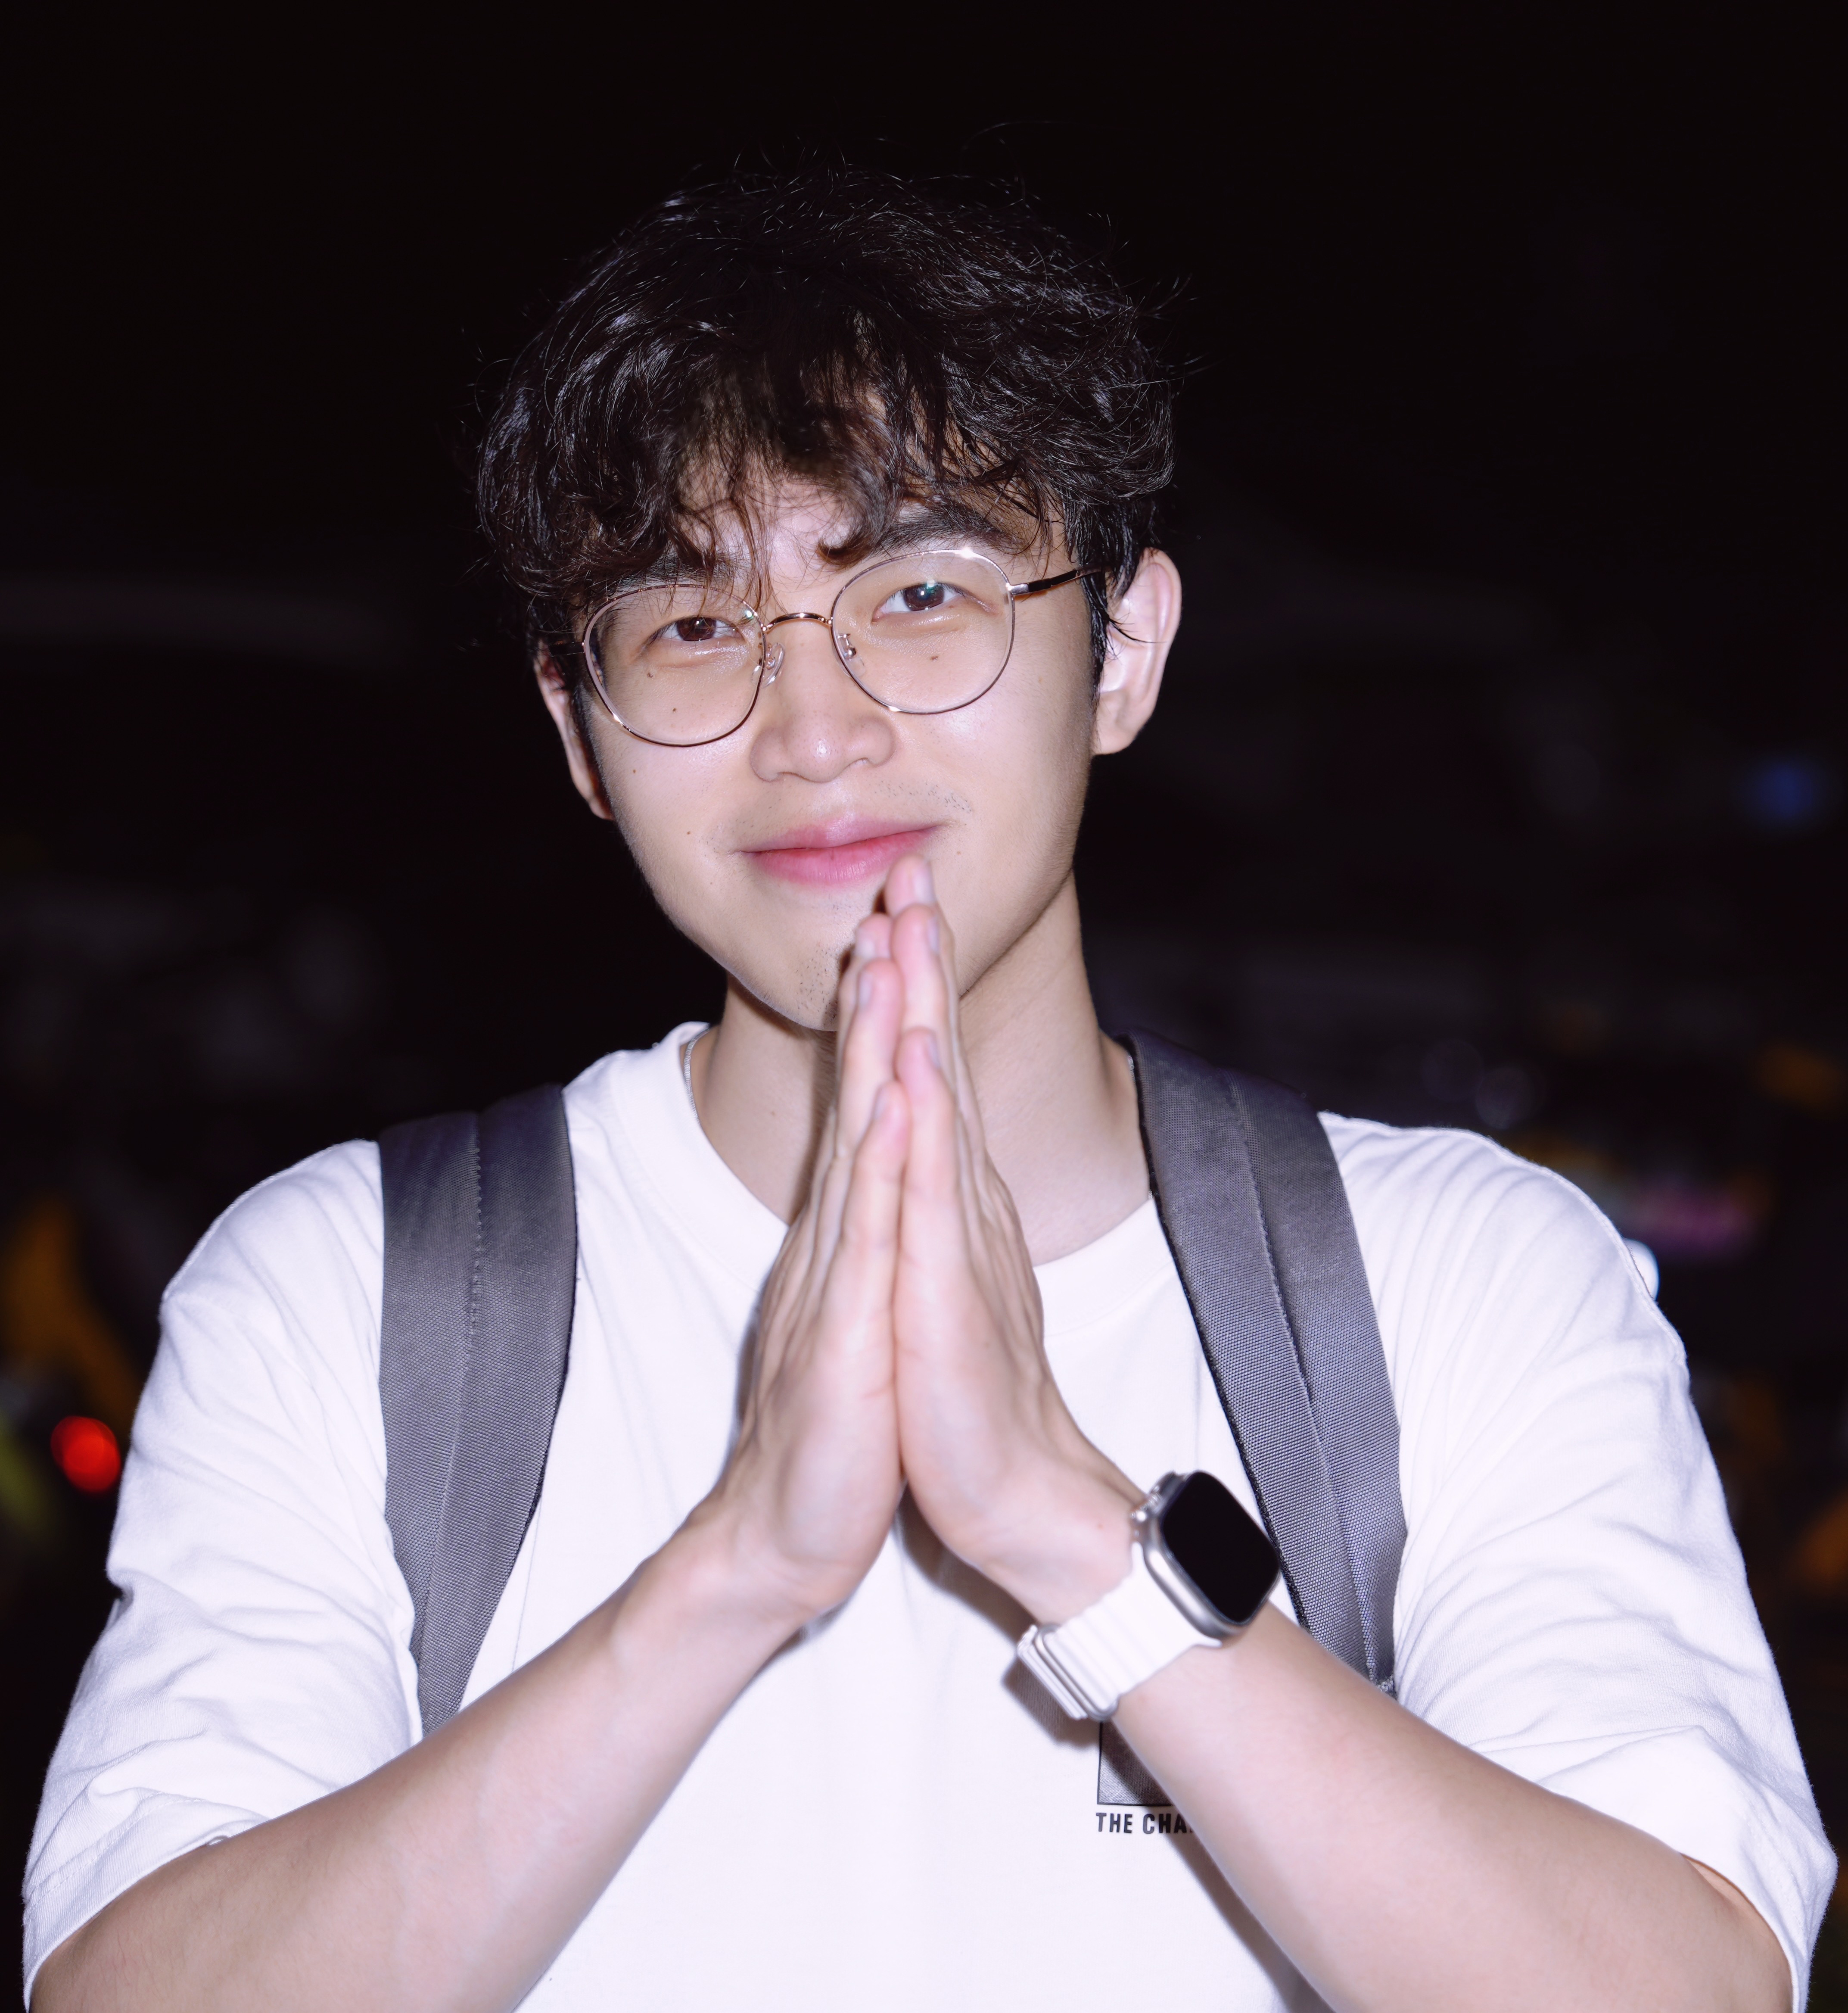
\includegraphics[height=4.5cm]{photo.jpg}% 把 mypic.jpg 换成你真实的照片文件
  \end{flushright}
\end{minipage}

% \vspace{0.5em}               % 2em 大小的垂直空白,可按需修改

 
\section{研究领域}
群智协同与系统优化、角色协同(Role-Based Collaboration)下的AI大模型演化。
\vspace{2pt}

\section{工作经历}
\datedsubsection{\textbf{广东工业大学},计算机学院,\textit{助理研究员}(合作导师:刘冬宁教授)}{2023.9 - 至今}
\begin{itemize}
  \item \textbf{[国家重点研发计划] 产业链协作企业群群体智能理论和服务方法(项目骨干)。}探究基于角色协同的产业链智能优化算法,(1)设计基于角色协同的GRAMAC模型,以最小化多Agent装配过程中的代理冲突;(2)寻找到多Agent装配无冲突的充分必要条件,以进一步压缩问题求解空间,以期加快精准指派速度;(3)通过比亚迪汽车产业链、小鸭家电产业链等企业脱敏数据验证所提出的原创模型与算法能大幅提高智能装配效率;(4)相关成果以\textbf{唯一第一作者}发表在控制系统顶级期刊\textbf{IEEE Transactions on Systems, Man, and Cybernetics: Systems (T-SMC)}。
\end{itemize}
\vspace{2pt}

\section{教育背景}
\datedsubsection{\textbf{澳门科技大学},智能科学与系统(全奖),\textit{工学博士}}{2021.9 - 2024.6}
\FancyBadge{teal}{THE 251-300}
\FancyBadge{red}{QS 464}\vspace{2pt}\newline
\textbf{导师}:伍乃骐教授(\textbf{IEEE Fellow})、乔岩副教授\newline
\ \textbf{排名1/100 (GPA 4.0/4.0)}、2024年度澳門博士研究生科技研發獎(\textbf{澳门科技大学理工科唯一获得者})。\vspace{2pt}
\datedsubsection{\textbf{广东工业大学},计算机科学与技术(保送),\textit{工学硕士}}{2018.9 - 2021.6}
\FancyBadge{teal}{THE 601-800}
\FancyBadge{magenta}{USN 586}\vspace{2pt}\newline
\textbf{导师}:朱海滨教授(\textbf{IEEE Fellow})、刘冬宁教授\newline
\ \textbf{国家奖学金},2021年获澳门科技大学\textbf{博士全额奖学金}。\vspace{2pt}
\datedsubsection{\textbf{加州大学圣地亚哥分校},工程与技术项目,\textit{广东工业大学交换生}}{2017.7 - 2017.8}
\FancyBadge{teal}{THE 34}
\FancyBadge{red}{QS 72}
\FancyBadge{magenta}{USN 21}\vspace{2pt}\newline
\ 2017年经广东工业大学推荐,参与\textbf{加州大学圣地亚哥分校(UCSD)}工程与技术海外研修项目。\vspace{2pt}
\datedsubsection{\textbf{广东工业大学},网络工程,\textit{工学学士}}{2014.9 - 2018.6}
\FancyBadge{teal}{THE 601-800}
\FancyBadge{magenta}{USN 586}\vspace{2pt}\newline
\textbf{导师}:朱海滨教授(\textbf{IEEE Fellow})、刘冬宁教授\newline
\ \textbf{排名3/200 (系第3),国家奖学金},2017年获广东工业大学计算机学院硕士研究生\textbf{推免资格}。
\vspace{2pt}


\section{科研成果}
\begin{enumerate}[leftmargin=1.5em, itemsep=1ex]

  \item \myname{Qian Jiang (唯一第一作者)}, Haibin Zhu, Yan Qiao, Zhiwei He, Dongning Liu*, Baoying Huang. 
        \emph{Agent Evaluation in Deployment of Multi-SUAVs for Communication Recovery.}  
        \textbf{IEEE Transactions on Systems, Man, and Cybernetics: Systems (T-SMC)}, 52(11): 6968–6982, 2022. 
        (\textbf{TOP期刊}, JCR Q1, IF: 8.6, CAA A类推荐期刊, \textbf{他引次数: 34})
        \PaperBoxLink{https://ieeexplore.ieee.org/abstract/document/9638713}
        \CodeBoxLink{https://github.com/jiangqian1997/E-CARGO-Codes}

  \item \myname{Qian Jiang (唯一第一作者)}, Dongning Liu, Haibin Zhu, Naiqi Wu, Baoying Huang,  Yan Qiao*. 
        \emph{Group Role Assignment with Minimized Agent Conflicts.}  
        \textbf{IEEE Transactions on Systems, Man, and Cybernetics: Systems (T-SMC)}, early access, doi: 10.1109/TSMC.2024.3510588. 
        (\textbf{TOP期刊}, JCR Q1, IF: 8.6, CAA A类推荐期刊)
        \PaperBoxLink{https://ieeexplore.ieee.org/document/10807250}
        \CodeBoxLink{https://github.com/jiangqian1997/E-CARGO-Codes}

  \item \myname{Qian Jiang (唯一第一作者)}, Dongning Liu, Haibin Zhu, Yan Qiao, Baoying Huang*. 
        \emph{Quasi Group Role Assignment with Role Awareness in Self-Service Spatiotemporal Crowdsourcing.}  
        \textbf{IEEE Transactions on Computational Social Systems (T-CSS)}, 9(5): 1456–1468, 2022. 
        (JCR Q1, IF: 4.5, CAA A类推荐期刊, \textbf{他引次数: 33})
        \PaperBoxLink{https://ieeexplore.ieee.org/abstract/document/9670447}
        \CodeBoxLink{https://github.com/jiangqian1997/E-CARGO-Codes}

  \item \myname{Qian Jiang (唯一第一作者)}, Haibin Zhu, Yan Qiao, Dongning Liu*, Baoying Huang. 
        \emph{Refugee Resettlement by Extending Group Multirole Assignment.}  
        \textbf{IEEE Transactions on Computational Social Systems (T-CSS)}, 10(1): 36–47, 2023. 
        (JCR Q1, IF: 4.5, CAA A类推荐期刊, \textbf{他引次数: 30})
        \PaperBoxLink{https://ieeexplore.ieee.org/abstract/document/9650702}
        \CodeBoxLink{https://github.com/jiangqian1997/E-CARGO-Codes}

  \item \myname{Qian Jiang (唯一第一作者)}, Haibin Zhu, Yan Qiao, Dongning Liu*, Baoying Huang. 
        \emph{Extending Group Role Assignment With Cooperation and Conflict Factors via KD45 Logic.}  
        \textbf{IEEE Transactions on Computational Social Systems (T-CSS)}, 10(1): 178-191, 2023. 
        (JCR Q1, IF: 4.5, CAA A类推荐期刊, \textbf{他引次数: 25})
        \PaperBoxLink{https://ieeexplore.ieee.org/abstract/document/9732178}
        \CodeBoxLink{https://github.com/jiangqian1997/E-CARGO-Codes}

  \item \myname{Qian Jiang (唯一第一作者)}, Dongning Liu, Haibin Zhu, Yan Qiao, Baoying Huang*. 
        \emph{Equilibrium Means Equity? An E-CARGO Perspective on the Golden Mean Principle.} 
        \textbf{IEEE Transactions on Computational Social Systems (T-CSS)}, 10(4): 1443-1454, 2023. 
        (JCR Q1, IF: 4.5, CAA A类推荐期刊, \textbf{他引次数: 14})
        \PaperBoxLink{https://ieeexplore.ieee.org/abstract/document/9802892}
        \CodeBoxLink{https://github.com/jiangqian1997/E-CARGO-Codes}

  \item \myname{Qian Jiang (唯一第一作者)}, Dongning Liu, Haibin Zhu, Shijue Wu, Naiqi Wu, Xin Luo, Yan Qiao*. 
        \emph{Iterative Role Negotiation via the Bi-level GRA++ with Decision Tolerance.}  
        \textbf{IEEE Transactions on Computational Social Systems (T-CSS)}, 11(6): 7484-7499, 2024. 
        (JCR Q1, IF: 4.5, CAA A类推荐期刊, \textbf{他引次数: 10})
        \PaperBoxLink{https://ieeexplore.ieee.org/document/10574173}
        \CodeBoxLink{https://github.com/jiangqian1997/E-CARGO-Codes/tree/main/Python_Code_for_GRA_NSGA_II_Algorithm}

  \item \myname{Qian Jiang (唯一第一作者)}, Dongning Liu, Haibin Zhu, Baoying Huang, Naiqi Wu, Yan Qiao*. 
        \emph{Quasi Group Role Assignment with Agent Satisfaction in Self-Service Spatiotemporal Crowdsourcing.}  
        \textbf{IEEE Transactions on Computational Social Systems (T-CSS)}, 11(5): 7002-7019, 2024.
        (JCR Q1, IF: 4.5, CAA A类推荐期刊, \textbf{他引次数: 2})
        \PaperBoxLink{https://ieeexplore.ieee.org/document/10595440}
        \CodeBoxLink{https://github.com/jiangqian1997/E-CARGO-Codes}

  \item \myname{Qian Jiang (唯一第一作者)}, Haibin Zhu, Fuyan Wen, Dongning Liu*, Naiqi Wu, Yan Qiao*. 
        \emph{Scheduling Multi-Evaporators in Cold Storage to Defrost: Handling Dynamic Defrosting Conflicts via GRA with Sliding Windows.}  
        \textbf{IEEE/CAA Journal of Automatica Sinica (IEEE/CAA JAS)}, Under Review.
        (JCR Q1, IF: 15.3, CAA A+类推荐期刊)
        \PaperBoxLink{https://jiangqian1997.github.io/}
        \CodeBoxLink{https://github.com/jiangqian1997/E-CARGO-Codes}

  \item \myname{Qian Jiang (唯一第一作者)}, Haibin Zhu, Ming Liao, Baoying Huang, XiaoZhao Fang, Dongning Liu*. 
        \emph{Solving the Signal Relay Problem of UAV in Disaster Relief via Group Role Assignment.}  
        \textbf{Proceeding of Computer Supported Cooperative Work and Social Computing (Chinese CSCW)}, 1042: 18-29, 2019.
        (EI会议, \textbf{他引次数: 2})
        \PaperBoxLink{https://link.springer.com/chapter/10.1007/978-981-15-1377-0_2}
        \CodeBoxLink{https://github.com/jiangqian1997/E-CARGO-Codes}

  \item Dongning Liu, \myname{Qian Jiang (学生第一作者)}, Haibin Zhu*, Baoying Huang. 
        \emph{Distributing UAVs as Wireless Repeaters in Disaster Relief via Group Role Assignment.}  
        \textbf{International Journal of Cooperative Information Systems (IJCIS)}, 29(1\&2): 2040002-1–22, 2020.
        (JCR Q4, IF: 0.5, CCF C类推荐期刊, \textbf{他引次数: 29})
        \PaperBoxLink{https://www.worldscientific.com/doi/abs/10.1142/S021884302040002X}
        \CodeBoxLink{https://github.com/jiangqian1997/E-CARGO-Codes}

  \item Baoying Huang, Haibin Zhu, Dongning Liu*, Naiqi Wu, Yan Qiao, \myname{Qian Jiang}. 
        \emph{Solving Last-Mile Logistics Problem in Spatiotemporal Crowdsourcing via Role Awareness With Adaptive Clustering.}  
        \textbf{IEEE Transactions on Computational Social Systems (T-CSS)}, 8(3): 668-681, 2021.
        (JCR Q1, IF: 4.5, CAA A类推荐期刊, \textbf{他引次数: 40})
        \PaperBoxLink{https://ieeexplore-ieee-org/document/9354439}
        \CodeBoxLink{https://github.com/jiangqian1997/E-CARGO-Codes}

  \item Haibin Zhu*, Dongning Liu, Hua Ma, Yin Sheng, Libo Zhang, \myname{Qian Jiang}. 
        \emph{E-CARGO/RBC Research Guide: A Road Map for Researchers.}  
        \textbf{IEEE Systems, Man, and Cybernetics Magazine (IEEE SMC Magazine)}, 10(3): 64-75, 2024.
        (JCR Q3, IF: 1.9, \textbf{他引次数: 4})
        \PaperBoxLink{https://ieeexplore.ieee.org/document/10592091}
        \CodeBoxLink{https://github.com/jiangqian1997/E-CARGO-Codes}
\end{enumerate}

% \vspace{0.3em}

\section{科研经历}
\datedsubsection{\textbf{[青年基金]复杂多维冲突下多对多指派算法及其协同优化(待主持)}}{预计2026.1-2028.12}
\begin{itemize}[itemsep=0.5ex]
  \item \textbf{任务描述}: 
    国家低空经济发展和灾害救援的紧迫需求下,应对业务流程复杂度骤增与多维冲突约束带来的挑战,现有的人机物协同系统优化策略陷入\textbf{建模泛化能力弱、求解精度低、自适应演化效率慢}等困境。亟需为实现复杂多维冲突下多对多任务的高效精准指派引入全新的理论框架与实践范式。
  \item \textbf{技术路线}: 
    (1)提出一种基于角色协同的三层可计算决策架构,通过对多维冲突约束下指派任务逐级抽象,以实现\textbf{集中式控制、分布式执行}的协同优化模型;
    (2)设计Σ2P与NP级指派算法,在保障计算精度的前提下,加速指派过程,降低算法的计算代价;
    (3)实现可视化交互仿真系统支持下的原型验证,推演协同决策的趋势与走向,进而获得协同资源自适应优化机制。
  \item \textbf{相关成果}: 
    (1)在真实数据集(如中国地震局深圳防灾减灾技术研究院提供的部分灾区灾情空天地数据)和企业脱敏数据集(如北方华创、小鹏汽车、美团等)上均达到最佳指派效果;  
    (2)相关工作已被系统控制类顶刊\textbf{T-SMC}、\textbf{T-CSS}接收。
\end{itemize}

\vspace{1pt}

\datedsubsection{\textbf{[面上项目]多无人机系统的多对多指派算法与协同优化(项目骨干)}}{2021.1-2024.12}
\begin{itemize}[itemsep=0.5ex]
  \item \textbf{任务描述}: 
    针对灾害救援中通信恢复的紧迫需求,提出一种基于多太阳能无人机(SUAV)的通信中继网络部署方案。为应对多约束复杂环境下的任务分配难题,解决现有路径规划算法在不确定路径和累积姿态误差场景下的局限性,亟需构建精准高效的多无人机协同部署理论框架。
  \item \textbf{技术路线}: 
    (1)提出基于群组角色多对多指派模型的扩展方法(UGRA),对多无人机部署中继通信问题进行形式化建模;
    (2)设计动态曲线路径规划算法(DCPPA)和贪心曲直路径规划算法(GCSPPA),以适应复杂环境中的路径规划需求,并通过充分与必要条件加速算法收敛;
    (3)通过大规模对比实验验证算法性能,支持基于UGRA模型的快速无人机分配和通信网络部署。
  \item \textbf{相关成果}: 
    (1)在真实数据集(如九寨沟救援场景高程数据集)下验证,结果表明提出的路径规划算法在复杂路径环境下显著优于传统算法(如Dijkstra、A*和改进的并行PSO算法),能够快速计算最优路径;
    (2)结合加速算法,UGRA模型可实现在分钟级时间内完成多无人机到中继点的快速分配;
    (3)提出的DCPPA算法和GCSPPA算法填补了\textbf{姿态误差动态校正下}无人机巡航研究的\textbf{领域空白};
    (4)相关工作已被系统控制类顶刊\textbf{T-SMC}及\textbf{IJCIS}接收。
\end{itemize}

\vspace{1pt}

\datedsubsection{\textbf{[校企合作]美团拍店:自助式众包任务指派及其均衡优化(项目骨干)}}{2022.1-至今}
\begin{itemize}[itemsep=0.5ex]
  \item \textbf{任务描述}: 
    社会5.0(Society 5.0)衍生出以人为本的任务众包指派新需求,而本项目聚焦于自助式时空众包(Self-serive Spatiotemporal Crowdsourcing)中存在的任务完成率低及工人满意度低等问题。针对此,研究以美团拍店为新型场景,分析任务完成率低、用户满意度低的原因,并设计众包任务均衡指派策略。
  \item \textbf{技术路线}: 
    (1) 提出基于任务聚类的角色感知(Role Awareness)方法,将任务划分为高利润任务簇,降低分配时间复杂度并提升任务完成率;
    (2)提出非饱和式群组角色指派模型(QGRA),引入了代理满意度过滤算法(SFA),通过筛选最优任务分配方案,提高工人满意度;
    (3)设计包含决策容忍度(Decision Tolerance)的GRA-NSGA-II算法,帮助决策者在多Pareto前沿解中选择当前需求下的最优解。
  \item \textbf{相关成果}: 
    (1) 在美团拍店app中部分脱敏数据集下验证,结果表明所提出的方法在保证任务完成率高达90\%的同时,使用户满意度提高100\%;
    (2)所提出的\textbf{GRA-NSGA-II算法}第一次将基于角色协同控制模型与智能算法联袂共融,实现模型-算法“\textbf{自上而下控制,自下而上演化}”;
    (3)相关工作已被系统控制类顶刊\textbf{T-CSS}接收。
\end{itemize}

\vspace{1pt}

\datedsubsection{\textbf{[校企合作]冷链物流下冷库多蒸发器系统动态除霜(项目骨干)}}{2023.1-至今}
\begin{itemize}[itemsep=0.5ex]
  \item \textbf{任务描述}: 
    冷库作为冷链物流的重要组成部分,随着冷链订单的增加,冷库设施长期满负荷运行,除霜成为冷库运营与维护的关键任务。然而,现有的除霜策略多依赖经验,容易导致蒸发器除霜时间不当,引发设备损坏,影响设施正常运行。本项目从\textbf{系统最优化}的角度,提出了一种冷库除霜的最优策略,旨在规避蒸发器除霜任务之间的动态冲突,同时实现最低的除霜操作总成本。
  \item \textbf{技术路线}: 
    (1) 利用多滑动窗口的概念表示\textbf{动态冲突},将冷库多蒸发器除霜调度(SMECS)问题简化为多滑动窗口的群体角色分配(GRASW)问题;
    (2)通过GRASW问题的形式化,大幅降低控制变量的维度及其相关约束,从而减少问题求解空间;
    (3)证明SMECS与GRASW问题的等价性,说明GRASW问题的解是SMECS问题无冲突最优解的\textbf{充分必要条件}。
  \item \textbf{相关成果}: 
    (1)基于广州市某大型冷库脱敏数据验证。实验表明,与现有方法相比,本文提出的解决方案不仅完全避免了蒸发器除霜任务之间的动态冲突,还将\textbf{工业电费成本降低约49.85\%};
    (2)基于优化模型生成的设计指南能够帮助冷库管理者构建更可靠、维护成本更低的蒸发器系统,为冷库设施的系统优化管理提供了一种全新的理论框架和实践工具;
    (3)相关工作已投稿至系统控制类顶刊\textbf{IEEE/CAA Journal of Automatica Sinica}。
\end{itemize}

\vspace{2pt}
\section{荣誉奖项}
% increase linespacing [parsep=0.5ex]
\begin{itemize}[parsep=0.3ex]
  \item \AwardBoxLink{https://www.fdct.gov.mo/zh_tw/fund_information_detail/article/m2itb3kz.html}{2024年度澳門博士研究生科技研發獎}\textbf{ :澳门博士生最高荣誉,每两年评选一次},评选范围为澳门(籍)博士生或近两年毕业的澳门(籍)博士,共20位获得者,\textbf{本人为澳门科技大学理工学科唯一获得者,奖金8万元};
  \item 2021年澳门科技大学智能科学与系统\textbf{博士全额奖学金};
  \item 2020年\textbf{华为技术有限公司}西安公共开发部AI工程师Offer;
  \item 2020年全国研究生数学建模竞赛三等奖;
  \item 2020年硕士研究生\textbf{国家奖学金};
  \item 2019年全国研究生数学建模竞赛三等奖;
  \item 2017年广东工业大学计算机学院硕士研究生\textbf{推免资格};
  \item 2017年本科生\textbf{国家奖学金};
  \item 2015年全国大学生英语竞赛C类三等奖,同年通过CET-6。
\end{itemize}

\vspace{2pt}
\section{学术服务}
% increase linespacing [parsep=0.5ex]
\begin{itemize}[parsep=0.3ex]
  \item \textbf{期刊/会议审稿人:} T-SMC,T-CSS,IEEE Transactions on Automation Science and Engineering (T-ASE), IEEE International Conference on ComputerSupported Cooperative Work in Design (IEEE CSCWD), and etc.;
  \item 2025 IEEE CSCWD, \textbf{Program Committee Member};
  \item 2025 IEEE International Summer School on E-CARGO and Applications,  \AwardBoxLink{http://www.e-cargoschool.com/\#/}{Tutorial Presenter};
  \item 2024 IEEE International Summer School on E-CARGO and Applications,  \AwardBoxLink{http://www.e-cargoschool.com/2/\#/}{Local Organization Co-Chair};
  \item 2023 IEEE International Summer School on E-CARGO and Applications,  \AwardBoxLink{http://www.e-cargoschool.com/1/\#/}{Lab Instructor};
  \item 2022 ChineseCSCW顶会顶刊论文交流论坛,\textbf{特邀讲者}。
\end{itemize}

\end{document}
